\documentclass{beamer}
\usepackage{amsmath}
\usepackage{amssymb}
\usepackage{graphicx}
\usepackage{xcolor}
\usepackage{listings}
\usepackage{algorithm}
\usepackage{algpseudocode}
\usepackage{tikz}
\usepackage{empheq}



% Define colors for JavaScript syntax highlighting
\definecolor{codegreen}{rgb}{0,0.6,0}
\definecolor{codegray}{rgb}{0.5,0.5,0.5}
\definecolor{codepurple}{rgb}{0.58,0,0.82}
\definecolor{backcolour}{rgb}{0.95,0.95,0.92}

% JavaScript code style
\lstdefinestyle{jsstyle}{
    backgroundcolor=\color{backcolour},   
    commentstyle=\color{codegreen},
    keywordstyle=\color{magenta},
    numberstyle=\tiny\color{codegray},
    stringstyle=\color{codepurple},
    basicstyle=\ttfamily\footnotesize,
    breakatwhitespace=false,         
    breaklines=true,                 
    captionpos=b,                    
    keepspaces=true,                 
    numbers=left,                    
    numbersep=5pt,                   
    showspaces=false,                
    showstringspaces=false,
    showtabs=false,                  
    tabsize=2,
    language=JavaScript
}

% Theme configuration
\usetheme{Madrid}
\usecolortheme{default}
\setbeamertemplate{navigation symbols}{}
\setbeamertemplate{footline}[frame number]
\date{}
\title{The Alternating Direction Implicit (ADI) Method}
\subtitle{A Numerical Approach for Solving 2D Diffusion Equations}
 
\begin{document}

\begin{frame}
    \titlepage
    \begin{equation*}
        \frac{\partial u}{\partial t} = D\left(\frac{\partial^2 u}{\partial x^2} + \frac{\partial^2 u}{\partial y^2}\right)
    \end{equation*}
\end{frame}

\begin{frame}{ Discretize the Domain}
    \begin{itemize}
        \onslide<2->{
            \item $u_{i,j}^k$ represents the approximation of $u(x_i, y_j, t_k)$
        }
        \onslide<3->{
            \item Space discretization: $(x_i, y_j)$ where $x_i = i\Delta x$  and $y_j = j\Delta y$ 

        }
        \onslide<4->{   
            \item Time discretization: $t_k = k\Delta t$ for $k = 0,1,...$

        }
    \end{itemize}

       \begin{figure}
        \onslide<1->{
            \centering
            \begin{minipage}{0.29\textwidth}
                \centering
                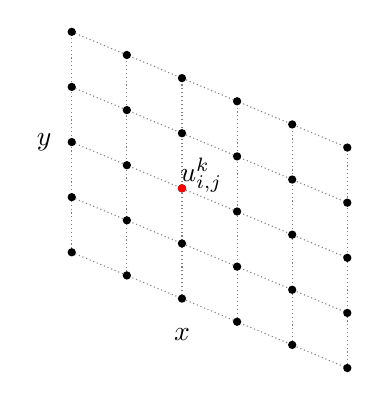
\begin{tikzpicture}[scale=0.7]
                    \foreach \y in {0,...,4}
                        \draw[gray, densely dotted] (0,\y) -- (5,\y-5*0.42);
                    
                    \foreach \x in {0,...,5}
                        \draw[gray, densely dotted] (\x,0-\x*0.42) -- (\x,4-\x*0.42);
                    
                    \foreach \x in {0,...,5}
                        \foreach \y in {0,...,4} {
                            \fill (\x,\y-\x*0.42) circle (0.0753);
                            \ifnum \x=2 \ifnum \y=2
                                \fill[red] (\x,\y-\x*0.42) circle (0.0753);
                            \fi \fi
                        }
                         
                          
                    \node at (2.0, -1.5) {$x$};
                    \node at (-0.5, 2) {$y$};
                    \node at (2.35, 1.4) {$u_{i,j}^k$};
                \end{tikzpicture}
            \end{minipage}
        }
        \onslide<5->{
            \hspace{0.4cm}
            \begin{minipage}{0.29\textwidth}
                \centering
                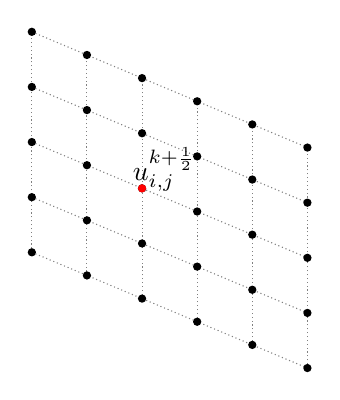
\begin{tikzpicture}[scale=0.7]
                    \foreach \y in {0,...,4}
                        \draw[gray, densely dotted] (0,\y) -- (5,\y-5*0.42);
                    
                    \foreach \x in {0,...,5}
                        \draw[gray, densely dotted] (\x,0-\x*0.42) -- (\x,4-\x*0.42);
                    
                        \foreach \x in {0,...,5}
                        \foreach \y in {0,...,4} {
                            \fill (\x,\y-\x*0.42) circle (0.0753);
                            \ifnum \x=2 \ifnum \y=2
                                \fill[red] (\x,\y-\x*0.42) circle (0.0753);
                            \fi \fi
                        }
                    
                    \node at (2.4, 1.5) {$u_{i,j}^{k+\frac{1}{2}}$};
                \end{tikzpicture}
            \end{minipage}
        }
        \onslide<4->{
            \begin{minipage}{0.29\textwidth}
                \centering
                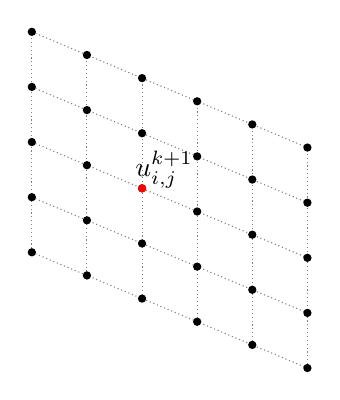
\begin{tikzpicture}[scale=0.7]
                    \foreach \y in {0,...,4}
                        \draw[gray, densely dotted] (0,\y) -- (5,\y-5*0.42);
                    
                    \foreach \x in {0,...,5}
                        \draw[gray, densely dotted] (\x,0-\x*0.42) -- (\x,4-\x*0.42);
                    
                        \foreach \x in {0,...,5}
                        \foreach \y in {0,...,4} {
                            \fill (\x,\y-\x*0.42) circle (0.0753);
                            \ifnum \x=2 \ifnum \y=2
                                \fill[red] (\x,\y-\x*0.42) circle (0.0753);
                            \fi \fi
                        } 
                            \node at (2.4, 1.5) {$u_{i,j}^{k+1}$};
                        \end{tikzpicture}
            \end{minipage}
            }
        \end{figure} 
        
        \begin{center}
        \begin{tikzpicture}[>=stealth]
            % Time arrow with specific steps
            \onslide<4->{
            \draw[->] (0,0) -- (11,0) node[label=above:Time] {};}
            
            % Time points and labels
            \onslide<4->{
            \fill (2,0) circle (0.1) node[below] {$k$};}
            \onslide<5->{
            \fill (5.5,0) circle (0.1) node[below] {$k+\frac{1}{2}$};}
            \onslide<4->{
            \fill (9,0) circle (0.1) node[below] {$k+1$};}
          
        \end{tikzpicture}
        \end{center}
\end{frame}

\begin{frame}{Discretize the diffusion equation}
    \begin{equation*}
        \frac{\partial u}{\partial t} = D\left(\frac{\partial^2 u}{\partial x^2} + \frac{\partial^2 u}{\partial y^2}\right)
    \end{equation*}


     \onslide<2->{
     \textbf{First half-step} ($x$ implicit, $y$ explicit):
     } 
    \begin{align*}
        \onslide<3->{\frac{u_{i,j}^{k+\frac{1}{2}} - u_{i,j}^k}{\Delta t/2} =} 
        \onslide<4->{D\left(
        \onslide<5->{    
        \frac{u_{i+1,j}^{k+\frac{1}{2}} - 2u_{i,j}^{k+\frac{1}{2}} + u_{i-1,j}^{k+\frac{1}{2}}}{\Delta x^2} }
            + 
        \onslide<6->{
            \frac{u_{i,j+1}^k - 2u_{i,j}^k + u_{i,j-1}^k}{\Delta y^2}
        }
            \right)} \nonumber \\
    \end{align*}
    \onslide<7->{
    \textbf{Second half-step} ($x$ explicit, $y$ implicit):
    }
    \begin{align*}
        \onslide<8->{\frac{u_{i,j}^{k+1} - u_{i,j}^{k+\frac{1}{2}}}{\Delta t/2} =} 
        \onslide<9->{D\left(
        \onslide<10->{    
        \frac{u_{i+1,j}^{k+\frac{1}{2}} - 2u_{i,j}^{k+\frac{1}{2}} + u_{i-1,j}^{k+\frac{1}{2}}}{\Delta x^2} }
            + 
        \onslide<11->{
            \frac{u_{i,j+1}^{k+1} - 2u_{i,j}^{k+1} + u_{i,j-1}^{k+1}}{\Delta y^2}
        }
            \right)} \nonumber \\
    \end{align*}

\end{frame}
\begin{frame}{Simplify the equation for the first half-step}
    % Define alpha at the top to save space
   
    \vspace{-0.5cm}
    \onslide<1->{
    % First equation
    \begin{align*}
     \frac{u_{i,j}^{k+\frac{1}{2}} - u_{i,j}^k}{\Delta t/2} &=
        D\left(   
        \frac{u_{i+1,j}^{k+\frac{1}{2}} - 2u_{i,j}^{k+\frac{1}{2}} + u_{i-1,j}^{k+\frac{1}{2}}}{\Delta x^2} 
            + 
            \frac{u_{i,j+1}^k - 2u_{i,j}^k + u_{i,j-1}^k}{\Delta y^2}
            \right)
    \end{align*}
    }
    \onslide<2->{
    \vspace{-0.3cm}
    Let's call $\alpha = \frac{D \Delta t}{2\Delta x^2}$
    \vspace{-0.2cm}
    }
   
    % Second equation (already simplified with alpha)
    \onslide<3->{
    \begin{align*}
    u_{i,j}^{k+\frac{1}{2}} - u_{i,j}^k &=
       \alpha 
       \left(   
       u_{i+1,j}^{k+\frac{1}{2}} - 2u_{i,j}^{k+\frac{1}{2}} + u_{i-1,j}^{k+\frac{1}{2}}
           + 
           u_{i,j+1}^k - 2u_{i,j}^k + u_{i,j-1}^k
           \right)
    \end{align*}
    }
    \onslide<4->{
    \vspace{-0.5cm}
   
    After simplifying, we get:
    }
    % Fourth equation (final form)
    \onslide<5->{
     \begin{align*}
        \boxed{
            \colorbox{red!20}{$ -\alpha u_{i-1,j}^{k+\frac{1}{2}} + (1 + 2\alpha)u_{i,j}^{k+\frac{1}{2}} - 
            \alpha u_{i+1,j}^{k+\frac{1}{2}} $}= 
            \colorbox{blue!20}{$\alpha u_{i,j-1}^k + (1 - 2\alpha)u_{i,j}^k + \alpha u_{i,j+1}^k$}}
    \end{align*}
    }
    % Fourth equation (final form)
    \onslide<6->{
    Where only three terms are unknown: $u_{i-1,j}^{k+\frac{1}{2}}$, $u_{i,j}^{k+\frac{1}{2}}$, and $u_{i+1,j}^{k+\frac{1}{2}}$
    }
    \vspace{-0.5cm}
  

\end{frame}

\begin{frame}{First half-step ($x$ implicit, $y$ explicit)}
    \vspace{-1cm}
    \begin{align*}
        \boxed{
            \colorbox{red!20}{$ -\alpha u_{i-1,j}^{k+\frac{1}{2}} + (1 + 2\alpha)u_{i,j}^{k+\frac{1}{2}} - 
            \alpha u_{i+1,j}^{k+\frac{1}{2}} $}= 
            \colorbox{blue!20}{$\alpha u_{i,j-1}^k + (1 - 2\alpha)u_{i,j}^k + \alpha u_{i,j+1}^k$}}
    \end{align*}
    \onslide<2->{
    \vspace{-0.5cm}
    Let's look around $i = 3$ and $j = 2$:
    \vspace{0.5cm}
    }
    \begin{figure}
            \centering
            \begin{minipage}{0.49\textwidth}
                \centering
                \onslide<3->{
                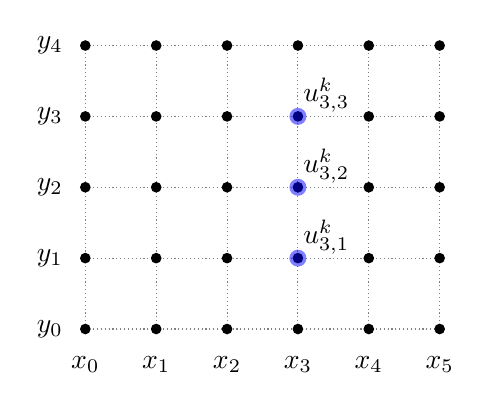
\begin{tikzpicture}[scale=0.9]
                   \foreach \y in {0,...,4} {
                        \draw[gray, densely dotted] (0,\y) -- (5,\y);
                        \node at (-0.5, \y) {$y_{\y}$};
                    }
                                        
                    \foreach \x in {0,...,5} {
                        \draw[gray, densely dotted] (\x,0) -- (\x,4);
                        \node at (\x, -0.5) {$x_{\x}$};
                    }
                    \foreach \x in {0,...,5}
                        \foreach \y in {0,...,4} {
                            \fill (\x,\y) circle (0.0753);
                           
                            \ifnum \x=3 \ifnum \y=1
                                \fill[blue,fill opacity=0.5 ] (\x,\y) circle (0.12);
                            \fi \fi
                            \ifnum \x=3 \ifnum \y=2
                                \fill[blue,fill opacity=0.5 ] (\x,\y) circle (0.12);
                            \fi \fi
                            \ifnum \x=3 \ifnum \y=3
                                \fill[blue,fill opacity=0.5 ] (\x,\y) circle (0.12);
                            \fi \fi
                        }
                    \node at (3.4, 2.3) {$u_{3,2}^k$};
                    \node at (3.4, 1.3) {$u_{3,1}^k$};
                    \node at (3.4, 3.3) {$u_{3,3}^k$};
                \end{tikzpicture}
                }
            \end{minipage}%
            \begin{minipage}{0.49\textwidth}
                \centering
                \onslide<4->{
                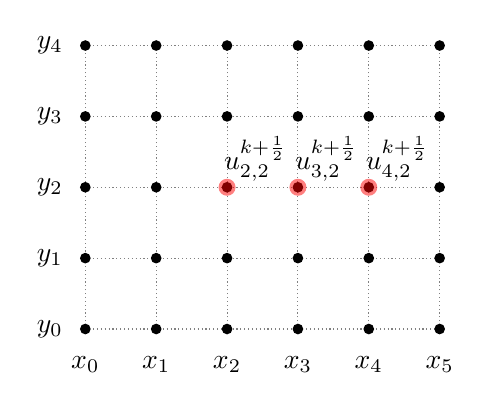
\begin{tikzpicture}[scale=0.9]
                    \foreach \y in {0,...,4} {
                        \draw[gray, densely dotted] (0,\y) -- (5,\y);
                        \node at (-0.5, \y) {$y_{\y}$};
                    }
                                        
                    \foreach \x in {0,...,5} {
                        \draw[gray, densely dotted] (\x,0) -- (\x,4);
                        \node at (\x, -0.5) {$x_{\x}$};
                    }
                    \foreach \x in {0,...,5}
                        \foreach \y in {0,...,4} {
                            \fill (\x,\y) circle (0.0753);
                          
                            \ifnum \x=3 \ifnum \y=2
                                \fill[red,fill opacity=0.5 ] (\x,\y) circle (0.12);
                            \fi \fi
                            \ifnum \x=2 \ifnum \y=2
                            \fill[red,fill opacity=0.5 ] (\x,\y) circle (0.12);
                        \fi \fi
                        \ifnum \x=4 \ifnum \y=2
                        \fill[red,fill opacity=0.5 ] (\x,\y) circle (0.12);
                    \fi \fi
                        }
                    \node at (3.4, 2.4) {$u_{3,2}^{k+\frac{1}{2}}$};
                    \node at (2.4, 2.4) {$u_{2,2}^{k+\frac{1}{2}}$};
                    \node at (4.4, 2.4) {$u_{4,2}^{k+\frac{1}{2}}$};
                \end{tikzpicture}
                }
            \end{minipage}
        \end{figure}
\end{frame}
\begin{frame}{Writing the tridiagonal matrix}
    \vspace{-0.8cm}   
    Let's fix $j = 1$ and write the equations for $i =  1, 2, 3, 4$:
    
    \begin{columns}
        \begin{column}{0.3\textwidth}
            % Place both figures in a row here
            \begin{minipage}{0.48\textwidth}
                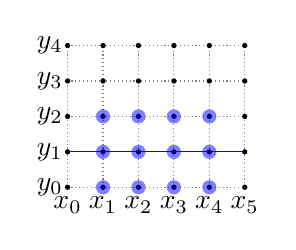
\begin{tikzpicture}[scale=0.45]
                    \foreach \y in {0,...,4} {
                         \draw[gray, densely dotted] (0,\y) -- (5,\y);
                         \node at (-0.5, \y) {$y_{\y}$};
                         \ifnum \y = 1
                            \draw[blue, thin] (0,1) -- (5,1);
                         \fi
                     }
                                         
                     \foreach \x in {0,...,5} {
                         \draw[gray, densely dotted] (\x,0) -- (\x,4);
                         \node at (\x, -0.5) {$x_{\x}$};
                     }
                     \foreach \x in {0,...,5}
                         \foreach \y in {0,...,4} {
                             \fill (\x,\y) circle (0.0753);
                             \onslide<3->{  
                             \ifnum \x=1 \ifnum \y=0
                                 \fill[blue, fill opacity=0.5] (\x,\y) circle (0.2);
                             \fi \fi
                             \ifnum \x=1\ifnum \y=1
                                 \fill[blue, fill opacity=0.5] (\x,\y) circle (0.2);
                             \fi \fi
                             \ifnum \x=1 \ifnum \y=2
                                 \fill[blue, fill opacity=0.5] (\x,\y) circle (0.2);
                             \fi \fi
                             }
                            \onslide<4->{
                                \ifnum \x=2 \ifnum \y=0
                                    \fill[blue, fill opacity=0.5] (\x,\y) circle (0.2);
                                \fi \fi
                                \ifnum \x=2\ifnum \y=1
                                    \fill[blue, fill opacity=0.5] (\x,\y) circle (0.2);
                                \fi \fi
                                \ifnum \x=2 \ifnum \y=2
                                    \fill[blue, fill opacity=0.5] (\x,\y) circle (0.2);
                                \fi \fi
                                }
                            \onslide<5->{
                                \ifnum \x=3 \ifnum \y=0
                                    \fill[blue, fill opacity=0.5] (\x,\y) circle (0.2);
                                \fi \fi
                                \ifnum \x=3\ifnum \y=1
                                    \fill[blue, fill opacity=0.5] (\x,\y) circle (0.2);
                                \fi \fi
                                \ifnum \x=3 \ifnum \y=2
                                    \fill[blue, fill opacity=0.5] (\x,\y) circle (0.2);
                                \fi \fi
                                }
                            \onslide<6->{
                                \ifnum \x=4 \ifnum \y=0
                                    \fill[blue, fill opacity=0.5] (\x,\y) circle (0.2);
                                \fi \fi
                                \ifnum \x=4\ifnum \y=1
                                    \fill[blue, fill opacity=0.5] (\x,\y) circle (0.2);
                                \fi \fi
                                \ifnum \x=4 \ifnum \y=2
                                    \fill[blue, fill opacity=0.5] (\x,\y) circle (0.2);
                                \fi \fi
                                }

                         }
                         
                 \end{tikzpicture}
                \end{minipage}\\
            \vspace{-0.2cm}
            \onslide<2->{
            \begin{center}
                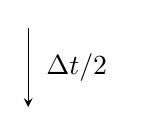
\begin{tikzpicture}[>=stealth]
                    \onslide<2->{
                    \draw[->] (0,0) -- (0,-1) node[midway, right, xshift=3pt] {$\Delta t/2$};}
                \end{tikzpicture}
            \end{center}
            \vspace{-0.2cm}
            \begin{minipage}{0.48\textwidth}
                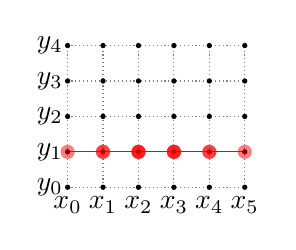
\begin{tikzpicture}[scale=0.45]
                    \foreach \y in {0,...,4} {
                         \draw[gray, densely dotted] (0,\y) -- (5,\y);
                         \node at (-0.5, \y) {$y_{\y}$};
                         \ifnum \y = 1
                         \draw[red, thin] (0,1) -- (5,1);
                      \fi
                     }
                                         
                     \foreach \x in {0,...,5} {
                         \draw[gray, densely dotted] (\x,0) -- (\x,4);
                         \node at (\x, -0.5) {$x_{\x}$};
                     }
                     \foreach \x in {0,...,5}
                         \foreach \y in {0,...,4} {
                             \fill (\x,\y) circle (0.0753);
                            \onslide<3->{
                             \ifnum \x=0 \ifnum \y=1
                                 \fill[red, fill opacity=0.5] (\x,\y) circle (0.2);
                             \fi \fi
                             \ifnum \x=1\ifnum \y=1
                                 \fill[red, fill opacity=0.5] (\x,\y) circle (0.2);
                             \fi \fi
                             \ifnum \x=2 \ifnum \y=1
                                 \fill[red, fill opacity=0.5] (\x,\y) circle (0.2);
                             \fi \fi
                         }
                         \onslide<4->{
                             \ifnum \x=1 \ifnum \y=1
                                 \fill[red, fill opacity=0.5] (\x,\y) circle (0.2);
                             \fi \fi
                             \ifnum \x=2\ifnum \y=1
                                 \fill[red, fill opacity=0.5] (\x,\y) circle (0.2);
                             \fi \fi
                             \ifnum \x=3 \ifnum \y=1
                                 \fill[red, fill opacity=0.5] (\x,\y) circle (0.2);
                             \fi \fi
                         }
                            \onslide<5->{
                                \ifnum \x=2 \ifnum \y=1
                                    \fill[red, fill opacity=0.5] (\x,\y) circle (0.2);
                                \fi \fi
                                \ifnum \x=3\ifnum \y=1
                                    \fill[red, fill opacity=0.5] (\x,\y) circle (0.2);
                                \fi \fi
                                \ifnum \x=4 \ifnum \y=1
                                    \fill[red, fill opacity=0.5] (\x,\y) circle (0.2);
                                \fi \fi
                            }
                            \onslide<6->{
                                \ifnum \x=3 \ifnum \y=1
                                    \fill[red, fill opacity=0.5] (\x,\y) circle (0.2);
                                \fi \fi
                                \ifnum \x=4\ifnum \y=1
                                    \fill[red, fill opacity=0.5] (\x,\y) circle (0.2);
                                \fi \fi
                                \ifnum \x=5 \ifnum \y=1
                                    \fill[red, fill opacity=0.5] (\x,\y) circle (0.2);
                                \fi \fi
                            }
                         
                         }
                \end{tikzpicture}
            \end{minipage}
            }
        \end{column}
        \hspace{-0.8cm}
       \begin{column}{0.7\textwidth}
            \footnotesize
            
            \vspace{-0.721cm}
            
            \onslide<3->{
            \begin{align*}
                -\alpha \textcolor{red}{u_{0,j}^{k+\frac{1}{2}}} + (1 + 2\alpha)\textcolor{red}{u_{1,j}^{k+\frac{1}{2}} }
                - \alpha \textcolor{red}{u_{2,j}^{k+\frac{1}{2}} }
                = \alpha \textcolor{blue}{u_{1,j-1}^k }
                + (1 - 2\alpha)\textcolor{blue}{u_{1,j}^k }
                + \alpha \textcolor{blue}{u_{1,j+1}^k}
            \end{align*}
            }
            \vspace{-0.721cm}
            \onslide<4->{
            \begin{align*}
                -\alpha \textcolor{red}{u_{1,j}^{k+\frac{1}{2}}} + (1 + 2\alpha)\textcolor{red}{u_{2,j}^{k+\frac{1}{2}} }
                - \alpha \textcolor{red}{u_{3,j}^{k+\frac{1}{2}} }
                = \alpha \textcolor{blue}{u_{2,j-1}^k }
                + (1 - 2\alpha)\textcolor{blue}{u_{2,j}^k }
                + \alpha \textcolor{blue}{u_{2,j+1}^k}
            \end{align*}
            }
            \vspace{-0.721cm}
            \onslide<5->{
            \begin{align*}
                -\alpha \textcolor{red}{u_{2,j}^{k+\frac{1}{2}}} + (1 + 2\alpha)\textcolor{red}{u_{3,j}^{k+\frac{1}{2}} }
                - \alpha \textcolor{red}{u_{4,j}^{k+\frac{1}{2}} }
                = \alpha \textcolor{blue}{u_{3,j-1}^k }
                + (1 - 2\alpha)\textcolor{blue}{u_{3,j}^k }
                + \alpha \textcolor{blue}{u_{3,j+1}^k}
            \end{align*}
            }
            \vspace{-0.721cm}
            \onslide<6->{
            \begin{align*}
                -\alpha \textcolor{red}{u_{3,j}^{k+\frac{1}{2}}} + (1 + 2\alpha)\textcolor{red}{u_{4,j}^{k+\frac{1}{2}} }
                - \alpha \textcolor{red}{u_{5,j}^{k+\frac{1}{2}} }
                = \alpha \textcolor{blue}{u_{4,j-1}^k }
                + (1 - 2\alpha)\textcolor{blue}{u_{4,j}^k }
                + \alpha \textcolor{blue}{u_{4,j+1}^k}
            \end{align*}
            }
            \vspace{-0.5cm}
            \onslide<7->{
            Which can be written as a matrix:
            }
            \vspace{-0.3cm}
            \onslide<8->{
                \begin{align*}
                    \begin{bmatrix}
                        -\alpha & 1 + 2\alpha & -\alpha & 0 & 0 & 0 \\
                        0 & -\alpha & 1 + 2\alpha & -\alpha & 0 & 0 \\
                        0 & 0 & -\alpha & 1 + 2\alpha & -\alpha & 0 \\
                        0 & 0 & 0 & -\alpha & 1 + 2\alpha & -\alpha \\
                    \end{bmatrix}
                    \begin{bmatrix}
                        \textcolor{red}{u_{0,j}^{k+\frac{1}{2}}} \\
                        \textcolor{red}{u_{1,j}^{k+\frac{1}{2}}} \\
                        \textcolor{red}{u_{2,j}^{k+\frac{1}{2}}} \\
                        \textcolor{red}{u_{3,j}^{k+\frac{1}{2}}} \\
                        \textcolor{red}{u_{4,j}^{k+\frac{1}{2}}} \\
                        \textcolor{red}{u_{5,j}^{k+\frac{1}{2}}}
                    \end{bmatrix}
                    =
                    \begin{bmatrix}
                        \textcolor{blue}{b_{1,j}} \\
                        \textcolor{blue}{b_{2,j}} \\
                        \textcolor{blue}{b_{3,j}} \\
                        \textcolor{blue}{b_{4,j}} \\
                    \end{bmatrix}
                \end{align*}
            Where $\textcolor{blue}{b_{i,j}}$ is the right hand side of the equation, which is already known.
            }
        \end{column}
    \end{columns}
\onslide<9->{
    \small
    Because of the boundary conditions, we can simplify the matrix to a tridiagonal matrix.
}
    \vspace{-1cm}
\end{frame}


\begin{frame}{Writing the tridiagonal matrix}
    \vspace{-0.8cm}   
    We get one system of equations for each $j$ value.
    
    \begin{columns}
        \begin{column}{0.3\textwidth}
            % Place both figures in a row here
            \begin{minipage}{0.48\textwidth}
                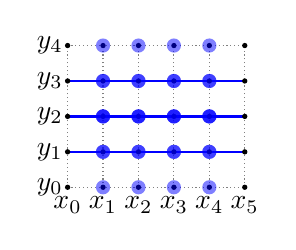
\begin{tikzpicture}[scale=0.45]
                    \foreach \y in {0,...,4} {
                         \draw[gray, densely dotted] (0,\y) -- (5,\y);
                         \node at (-0.5, \y) {$y_{\y}$};
                         \onslide<2->{
                         \ifnum \y = 1
                         \draw[blue, thick] (0,1) -- (5,1);
                      \fi
                         }
                         \onslide<3->{
                            \ifnum \y = 2
                            \draw[blue, thick] (0,2) -- (5,2);
                            \fi
                         }
                         \onslide<4->{
                            \ifnum \y = 3
                            \draw[blue, thick] (0,3) -- (5,3);
                            \fi
                         }
                     } 
                                         
                     \foreach \x in {0,...,5} {
                         \draw[gray, densely dotted] (\x,0) -- (\x,4);
                         \node at (\x, -0.5) {$x_{\x}$};
                     }
                     \foreach \x in {0,...,5}
                         \foreach \y in {0,...,4} {
                             \fill (\x,\y) circle (0.0753); 
                             \onslide<2->{
                             \ifnum  \y=1 \ifnum  \x>0 \ifnum  \x<5
                                 \fill[blue, fill opacity=0.5] (\x,\y) circle (0.2);
                            \fi \fi \fi
                            \ifnum  \y=2  \ifnum  \x>0 \ifnum  \x<5
                                \fill[blue, fill opacity=0.5] (\x,\y) circle (0.2);
                                \fi \fi \fi
                            \ifnum  \y=0 \ifnum  \x>0 \ifnum  \x<5
                                \fill[blue, fill opacity=0.5] (\x,\y) circle (0.2);
                                \fi \fi \fi 
                             }
                             \onslide<3->{
                                \ifnum  \y=1 \ifnum  \x>0 \ifnum  \x<5
                                    \fill[blue, fill opacity=0.5] (\x,\y) circle (0.2);
                                \fi \fi \fi
                                \ifnum  \y=2  \ifnum  \x>0 \ifnum  \x<5
                                    \fill[blue, fill opacity=0.5] (\x,\y) circle (0.2);
                                    \fi \fi \fi
                                \ifnum  \y=3 \ifnum  \x>0 \ifnum  \x<5
                                    \fill[blue, fill opacity=0.5] (\x,\y) circle (0.2);
                                    \fi \fi \fi 
                                 }
                           \onslide<4->{
                                \ifnum  \y=2 \ifnum  \x>0 \ifnum  \x<5
                                    \fill[blue, fill opacity=0.5] (\x,\y) circle (0.2);
                                \fi \fi \fi
                                \ifnum  \y=3  \ifnum  \x>0 \ifnum  \x<5
                                    \fill[blue, fill opacity=0.5] (\x,\y) circle (0.2);
                                    \fi \fi \fi
                                \ifnum  \y=4 \ifnum  \x>0 \ifnum  \x<5
                                    \fill[blue, fill opacity=0.5] (\x,\y) circle (0.2);
                                    \fi \fi \fi 
                                 


                           }
                         }
                         
                 \end{tikzpicture}
                \end{minipage}\\
            \vspace{-0.2cm}
           
            \begin{center}
                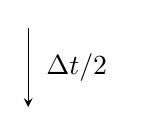
\begin{tikzpicture}[>=stealth]
                    \draw[->] (0,0) -- (0,-1) node[midway, right, xshift=3pt] {$\Delta t/2$};
                \end{tikzpicture}
            \end{center}
            \vspace{-0.2cm}
            \begin{minipage}{0.48\textwidth}
                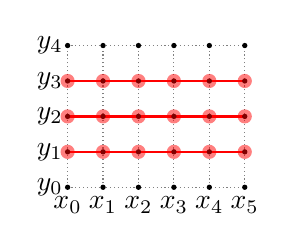
\begin{tikzpicture}[scale=0.45]
                    \foreach \y in {0,...,4} {
                         \draw[gray, densely dotted] (0,\y) -- (5,\y);
                         \node at (-0.5, \y) {$y_{\y}$};
                         \onslide<2->{
                         \ifnum \y = 1
                         \draw[red, thick] (0,1) -- (5,1);
                      \fi}
                        \onslide<3->{
                            \ifnum \y = 2
                            \draw[red, thick] (0,2) -- (5,2);
                            \fi
                        }
                        \onslide<4->{
                            \ifnum \y = 3
                            \draw[red, thick] (0,3) -- (5,3);
                            \fi
                        }
                     }
                                         
                     \foreach \x in {0,...,5} {
                         \draw[gray, densely dotted] (\x,0) -- (\x,4);
                         \node at (\x, -0.5) {$x_{\x}$};

                     }
                     \foreach \x in {0,...,5}
                         \foreach \y in {0,...,4} {
                             \fill (\x,\y) circle (0.0753); 
                             \onslide<2->{
                             \ifnum \y=1
                            \fill[red, fill opacity=0.5] (\x,\y) circle (0.2);
                            \fi
                            }
                            \onslide<3->{
                                \ifnum \y=2
                                \fill[red, fill opacity=0.5] (\x,\y) circle (0.2);
                                \fi
                            }
                            \onslide<4->{
                                \ifnum \y=3
                                \fill[red, fill opacity=0.5] (\x,\y) circle (0.2);
                                \fi
                            }
                         }
                \end{tikzpicture}
            \end{minipage}
            
        \end{column}
        \hspace{-0.8cm}
       \begin{column}{0.7\textwidth}
            %\footnotesize
            %we need smaller font size. let's try even smaller. Let's try tiny.
            \tiny
          \vspace{-1.5cm}  
          \onslide<2->{
                \begin{align*}
                    \begin{bmatrix}
                        1 + 2\alpha & -\alpha & 0 & 0  \\
                         -\alpha & 1 + 2\alpha & -\alpha & 0 \\
                        0 & -\alpha & 1 + 2\alpha & -\alpha  \\
                         0 & 0 & -\alpha & 1 + 2\alpha \\
                    \end{bmatrix}
                    \begin{bmatrix}
                        \textcolor{red}{u_{1,1}^{k+\frac{1}{2}}} \\
                        \textcolor{red}{u_{2,1}^{k+\frac{1}{2}}} \\
                        \textcolor{red}{u_{3,1}^{k+\frac{1}{2}}} \\
                        \textcolor{red}{u_{4,1}^{k+\frac{1}{2}}} \\
                    \end{bmatrix}
                    =
                    \begin{bmatrix}
                        \textcolor{blue}{b_{1,1}} \\
                        \textcolor{blue}{b_{2,1}} \\
                        \textcolor{blue}{b_{3,1}} \\
                        \textcolor{blue}{b_{4,1}} \\
                    \end{bmatrix}
                \end{align*}
          }
                \vspace{-0.5cm}
                \onslide<3->{
                \begin{align*}
                    \begin{bmatrix}
                        1 + 2\alpha & -\alpha & 0 & 0 \\
                         -\alpha & 1 + 2\alpha & -\alpha & 0  \\
                        0 & -\alpha & 1 + 2\alpha & -\alpha  \\
                         0 & 0 & -\alpha & 1 + 2\alpha  \\
                    \end{bmatrix}
                    \begin{bmatrix}
                        \textcolor{red}{u_{1,2}^{k+\frac{1}{2}}} \\
                        \textcolor{red}{u_{2,2}^{k+\frac{1}{2}}} \\
                        \textcolor{red}{u_{3,2}^{k+\frac{1}{2}}} \\
                        \textcolor{red}{u_{4,2}^{k+\frac{1}{2}}} \\
                    \end{bmatrix}
                    =
                    \begin{bmatrix}
                        \textcolor{blue}{b_{1,2}} \\
                        \textcolor{blue}{b_{2,2}} \\
                        \textcolor{blue}{b_{3,2}} \\
                        \textcolor{blue}{b_{4,2}} \\
                    \end{bmatrix}
                \end{align*}
                }
                \vspace{-0.5cm}
                \onslide<4->{
                \begin{align*}
                    \begin{bmatrix}
                        1 + 2\alpha & -\alpha & 0 & 0 \\
                         -\alpha & 1 + 2\alpha & -\alpha & 0  \\
                        0 & -\alpha & 1 + 2\alpha & -\alpha \\
                         0 & 0 & -\alpha & 1 + 2\alpha  \\
                    \end{bmatrix}
                    \begin{bmatrix}
                        \textcolor{red}{u_{1,3}^{k+\frac{1}{2}}} \\
                        \textcolor{red}{u_{2,3}^{k+\frac{1}{2}}} \\
                        \textcolor{red}{u_{3,3}^{k+\frac{1}{2}}} \\
                        \textcolor{red}{u_{4,3}^{k+\frac{1}{2}}} \\
                    \end{bmatrix}
                    =
                    \begin{bmatrix}
                        \textcolor{blue}{b_{1,3}} \\
                        \textcolor{blue}{b_{2,3}} \\
                        \textcolor{blue}{b_{3,3}} \\
                        \textcolor{blue}{b_{4,3}} \\
                    \end{bmatrix}
                \end{align*}
                }
                \vspace{-1.5cm}
        \end{column}
    \end{columns}
   
    \vspace{0.1cm}
    \small
    \onslide<5->{
        Now we can use the Thomas algorithm for solving each tridiagonal system.
    }
\end{frame}

\begin{frame}
That was the first half-step. Now we need to solve the second half-step.
\end{frame}

\begin{frame}{Simplify the equation for the second half-step}
    \vspace{-0.5cm}
    \onslide<1->{
    % Second half-step equation
    \begin{align*}
     \frac{u_{i,j}^{k+1} - u_{i,j}^{k+\frac{1}{2}}}{\Delta t/2} &=
        D\left(   
        \frac{u_{i+1,j}^{k+\frac{1}{2}} - 2u_{i,j}^{k+\frac{1}{2}} + u_{i-1,j}^{k+\frac{1}{2}}}{\Delta x^2} 
            + 
            \frac{u_{i,j+1}^{k+1} - 2u_{i,j}^{k+1} + u_{i,j-1}^{k+1}}{\Delta y^2}
            \right)
    \end{align*}
    }
    \onslide<2->{
    \vspace{-0.3cm}
    Let's call $\alpha = \frac{D \Delta t}{2\Delta y^2}$
    \vspace{-0.2cm}
    }
   
    % Simplified equation
    \onslide<3->{
    \begin{align*}
    u_{i,j}^{k+1} - u_{i,j}^{k+\frac{1}{2}} &=
       \alpha 
       \left(   
       u_{i+1,j}^{k+\frac{1}{2}} - 2u_{i,j}^{k+\frac{1}{2}} + u_{i-1,j}^{k+\frac{1}{2}}
           + 
           u_{i,j+1}^{k+1} - 2u_{i,j}^{k+1} + u_{i,j-1}^{k+1}
           \right)
    \end{align*}
    }
    \onslide<4->{
    \vspace{-0.5cm}
   
    After simplifying, we get:
    }
    % Final form
    \onslide<5->{
     \begin{align*}
        \boxed{
            \colorbox{red!20}{$ -\alpha u_{i,j-1}^{k+1} + (1 + 2\alpha)u_{i,j}^{k+1} - 
            \alpha u_{i,j+1}^{k+1} $}= 
            \colorbox{blue!20}{$\alpha u_{i-1,j}^{k+\frac{1}{2}} + (1 - 2\alpha)u_{i,j}^{k+\frac{1}{2}} + \alpha u_{i+1,j}^{k+\frac{1}{2}}$}}
    \end{align*}
    }
    % Explanation
    \onslide<6->{
    Where only three terms are unknown: $u_{i,j-1}^{k+1}$, $u_{i,j}^{k+1}$, and $u_{i,j+1}^{k+1}$
    }
    \vspace{-0.5cm}
\end{frame}

\begin{frame}{Second half-step ($x$ explicit, $y$ implicit)}
    \vspace{-1cm}
    \begin{align*}
        \boxed{
            \colorbox{red!20}{$ -\alpha u_{i,j-1}^{k+1} + (1 + 2\alpha)u_{i,j}^{k+1} - 
            \alpha u_{i,j+1}^{k+1} $}= 
            \colorbox{blue!20}{$\alpha u_{i-1,j}^{k+\frac{1}{2}} + (1 - 2\alpha)u_{i,j}^{k+\frac{1}{2}} + \alpha u_{i+1,j}^{k+\frac{1}{2}}$}}
    \end{align*}
    \onslide<2->{
    \vspace{-0.5cm}
    Let's look around $i = 3$ and $j = 2$:
    \vspace{0.5cm}
    }
    \begin{figure}
        \centering
        \begin{minipage}{0.49\textwidth}
            \centering
            \onslide<3->{
                    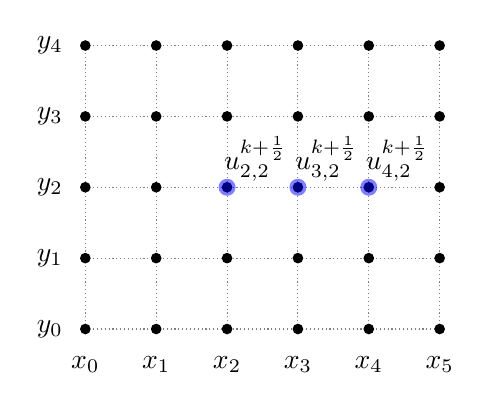
\begin{tikzpicture}[scale=0.9]
                        \foreach \y in {0,...,4} {
                            \draw[gray, densely dotted] (0,\y) -- (5,\y);
                            \node at (-0.5, \y) {$y_{\y}$};
                        }
                                            
                        \foreach \x in {0,...,5} {
                            \draw[gray, densely dotted] (\x,0) -- (\x,4);
                            \node at (\x, -0.5) {$x_{\x}$};
                        }
                        \foreach \x in {0,...,5}
                            \foreach \y in {0,...,4} {
                                \fill (\x,\y) circle (0.0753);
                              
                                \ifnum \x=3 \ifnum \y=2
                                    \fill[blue,fill opacity=0.5 ] (\x,\y) circle (0.12);
                                \fi \fi
                                \ifnum \x=2 \ifnum \y=2
                                \fill[blue,fill opacity=0.5 ] (\x,\y) circle (0.12);
                            \fi \fi
                            \ifnum \x=4 \ifnum \y=2
                            \fill[blue,fill opacity=0.5 ] (\x,\y) circle (0.12);
                        \fi \fi
                            }
                        \node at (3.4, 2.4) {$u_{3,2}^{k+\frac{1}{2}}$};
                        \node at (2.4, 2.4) {$u_{2,2}^{k+\frac{1}{2}}$};
                        \node at (4.4, 2.4) {$u_{4,2}^{k+\frac{1}{2}}$};
                    \end{tikzpicture}
                    }
                \end{minipage}
        \begin{minipage}
            {0.49\textwidth}
            \centering
            \onslide<4->{
                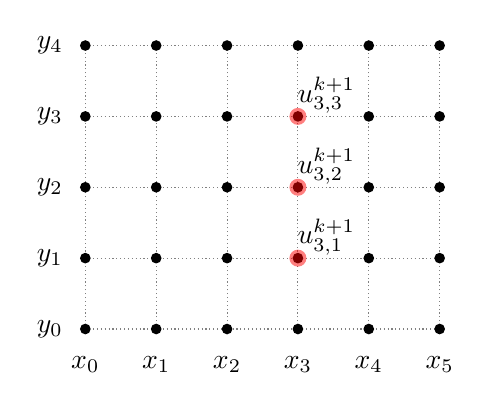
\begin{tikzpicture}[scale=0.9]
                    \foreach \y in {0,...,4} {
                         \draw[gray, densely dotted] (0,\y) -- (5,\y);
                         \node at (-0.5, \y) {$y_{\y}$};
                     }
                                         
                     \foreach \x in {0,...,5} {
                         \draw[gray, densely dotted] (\x,0) -- (\x,4);
                         \node at (\x, -0.5) {$x_{\x}$};
                     }
                     \foreach \x in {0,...,5}
                         \foreach \y in {0,...,4} {
                             \fill (\x,\y) circle (0.0753);
                            
                             \ifnum \x=3 \ifnum \y=1
                                 \fill[red,fill opacity=0.5 ] (\x,\y) circle (0.12);
                             \fi \fi
                             \ifnum \x=3 \ifnum \y=2
                                 \fill[red,fill opacity=0.5 ] (\x,\y) circle (0.12);
                             \fi \fi
                             \ifnum \x=3 \ifnum \y=3
                                 \fill[red,fill opacity=0.5 ] (\x,\y) circle (0.12);
                             \fi \fi
                         }
                     \node at (3.4, 2.3) {$u_{3,2}^{k+1}$};
                        \node at (3.4, 1.3) {$u_{3,1}^{k+1}$};
                        \node at (3.4, 3.3) {$u_{3,3}^{k+1}$};
                 \end{tikzpicture}
                 }
                
            \end{minipage}

        \end{figure}
\end{frame}
\begin{frame}{Writing the tridiagonal matrix}
    \vspace{-0.8cm}   
    Let's fix $i = 1$ and write the equations for $j =  1, 2, 3$:
    
    \begin{columns}
        \begin{column}{0.3\textwidth}
            % Place both figures in a row here
            \begin{minipage}{0.48\textwidth}
                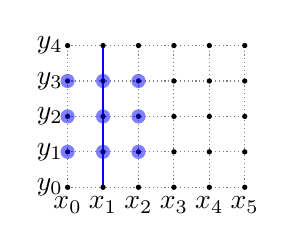
\begin{tikzpicture}[scale=0.45]
                    \foreach \y in {0,...,4} {
                         \draw[gray, densely dotted] (0,\y) -- (5,\y);
                         \node at (-0.5, \y) {$y_{\y}$};
                     }
                                         
                     \foreach \x in {0,...,5} {
                         \draw[gray, densely dotted] (\x,0) -- (\x,4);
                         \node at (\x, -0.5) {$x_{\x}$};
                         \onslide<1->{
                         \ifnum \x = 1
                            \draw[blue, thin] (1,0) -- (1,4);
                         \fi
                         }
                  
                     }
                     \foreach \x in {0,...,5}
                         \foreach \y in {0,...,4} {
                             \fill (\x,\y) circle (0.0753);
                             \onslide<3->{  
                             \ifnum \x=1 \ifnum \y=1
                                 \fill[blue, fill opacity=0.5] (\x,\y) circle (0.2);
                             \fi \fi
                             \ifnum \x=0\ifnum \y=1
                                 \fill[blue, fill opacity=0.5] (\x,\y) circle (0.2);
                             \fi \fi
                             \ifnum \x=2 \ifnum \y=1
                                 \fill[blue, fill opacity=0.5] (\x,\y) circle (0.2);
                             \fi \fi
                             }
                            \onslide<4->{
                                \ifnum \x=0 \ifnum \y=2
                                    \fill[blue, fill opacity=0.5] (\x,\y) circle (0.2);
                                \fi \fi
                                \ifnum \x=1\ifnum \y=2
                                    \fill[blue, fill opacity=0.5] (\x,\y) circle (0.2);
                                \fi \fi
                                \ifnum \x=2 \ifnum \y=2
                                    \fill[blue, fill opacity=0.5] (\x,\y) circle (0.2);
                                \fi \fi
                                }
                            \onslide<5->{
                             \ifnum \x=0 \ifnum \y=3
                                 \fill[blue, fill opacity=0.5] (\x,\y) circle (0.2);
                             \fi \fi
                                \ifnum \x=1\ifnum \y=3
                                    \fill[blue, fill opacity=0.5] (\x,\y) circle (0.2);
                                \fi \fi
                                \ifnum \x=2 \ifnum \y=3
                                    \fill[blue, fill opacity=0.5] (\x,\y) circle (0.2);
                                \fi \fi
                            }
                         }
                         
                 \end{tikzpicture}
                \end{minipage}\\
            \vspace{-0.2cm}
            \onslide<2->{
            \begin{center}
                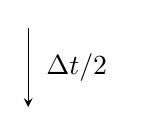
\begin{tikzpicture}[>=stealth]
                    \onslide<2->{
                    \draw[->] (0,0) -- (0,-1) node[midway, right, xshift=3pt] {$\Delta t/2$};}
                \end{tikzpicture}
            \end{center}
            \vspace{-0.2cm}
            \begin{minipage}{0.48\textwidth}
                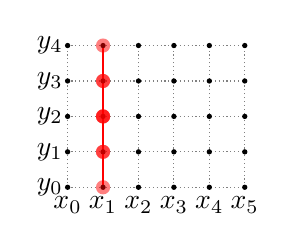
\begin{tikzpicture}[scale=0.45]
                    \foreach \y in {0,...,4} {
                         \draw[gray, densely dotted] (0,\y) -- (5,\y);
                         \node at (-0.5, \y) {$y_{\y}$};
                     }
                                         
                     \foreach \x in {0,...,5} {
                         \draw[gray, densely dotted] (\x,0) -- (\x,4);
                         \node at (\x, -0.5) {$x_{\x}$};
                         \onslide<2->{
                         \ifnum \x = 1
                            \draw[red, thin] (1,0) -- (1,4);
                         \fi
                         }
                     
                      
                     }
                     \foreach \x in {0,...,5}
                         \foreach \y in {0,...,4} {
                             \fill (\x,\y) circle (0.0753);
                            \onslide<3->{
                             \ifnum \x=1 \ifnum \y=0
                                 \fill[red, fill opacity=0.5] (\x,\y) circle (0.2);
                             \fi \fi
                             \ifnum \x=1\ifnum \y=1
                                 \fill[red, fill opacity=0.5] (\x,\y) circle (0.2);
                             \fi \fi
                             \ifnum \x=1 \ifnum \y=2
                                 \fill[red, fill opacity=0.5] (\x,\y) circle (0.2);
                             \fi \fi
                            
                         }
                         \onslide<4->{
                             \ifnum \x=1 \ifnum \y=1
                                 \fill[red, fill opacity=0.5] (\x,\y) circle (0.2);
                             \fi \fi
                             \ifnum \x=1\ifnum \y=2
                                 \fill[red, fill opacity=0.5] (\x,\y) circle (0.2);
                             \fi \fi
                             \ifnum \x=1 \ifnum \y=3
                                 \fill[red, fill opacity=0.5] (\x,\y) circle (0.2);
                             \fi \fi
                         
                         }
                            \onslide<5->{
                                \ifnum \x=1 \ifnum \y=2
                                    \fill[red, fill opacity=0.5] (\x,\y) circle (0.2);
                                \fi \fi
                                \ifnum \x=1\ifnum \y=3
                                    \fill[red, fill opacity=0.5] (\x,\y) circle (0.2);
                                \fi \fi
                                \ifnum \x=1 \ifnum \y=4
                                    \fill[red, fill opacity=0.5] (\x,\y) circle (0.2);
                                \fi \fi
                           
                            }
                         
                         }
                \end{tikzpicture}
            \end{minipage}
            }
        \end{column}
        \hspace{-0.8cm}
       \begin{column}{0.7\textwidth}
            \footnotesize
            
            \vspace{-0.721cm}
            
            \onslide<3->{
            \begin{align*}
                -\alpha \textcolor{red}{u_{1,0}^{k+1}} + (1 + 2\alpha)\textcolor{red}{u_{1,1}^{k+1}} 
                - \alpha \textcolor{red}{u_{1,2}^{k+1}}
                = \alpha \textcolor{blue}{u_{0,1}^{k+\frac{1}{2}}}
                + (1 - 2\alpha)\textcolor{blue}{u_{1,1}^{k+\frac{1}{2}}}
                + \alpha \textcolor{blue}{u_{2,1}^{k+\frac{1}{2}}}
            \end{align*}
            }
            \vspace{-0.721cm}
            \onslide<4->{
            \begin{align*}
                -\alpha \textcolor{red}{u_{1,1}^{k+1}} + (1 + 2\alpha)\textcolor{red}{u_{1,2}^{k+1}}
                - \alpha \textcolor{red}{u_{1,3}^{k+1}}
                = \alpha \textcolor{blue}{u_{0,2}^{k+\frac{1}{2}}}
                + (1 - 2\alpha)\textcolor{blue}{u_{1,2}^{k+\frac{1}{2}}}
                + \alpha \textcolor{blue}{u_{2,2}^{k+\frac{1}{2}}}
            \end{align*}
            }
            \vspace{-0.721cm}
            \onslide<5->{
            \begin{align*}
                -\alpha \textcolor{red}{u_{1,2}^{k+1}} + (1 + 2\alpha)\textcolor{red}{u_{1,3}^{k+1}}
                - \alpha \textcolor{red}{u_{1,4}^{k+1}}
                = \alpha \textcolor{blue}{u_{0,3}^{k+\frac{1}{2}}}
                + (1 - 2\alpha)\textcolor{blue}{u_{1,3}^{k+\frac{1}{2}}}
                + \alpha \textcolor{blue}{u_{2,3}^{k+\frac{1}{2}}}
            \end{align*}
            }
            \vspace{-0.5cm}
            \onslide<6->{
            Which can be written as a matrix:
            }
            \vspace{0.5cm}
            \onslide<7->{
                \begin{align*}
                    \begin{bmatrix}
                        -\alpha & 1 + 2\alpha & -\alpha & 0 & 0  \\
                        0 & -\alpha & 1 + 2\alpha & -\alpha & 0  \\
                        0 &0 & -\alpha & 1 + 2\alpha & -\alpha  \\
                    \end{bmatrix}
                    \begin{bmatrix}
                        \textcolor{red}{u_{1,0}^{k+1}} \\
                        \textcolor{red}{u_{1,1}^{k+1}} \\
                        \textcolor{red}{u_{1,2}^{k+1}} \\
                        \textcolor{red}{u_{1,3}^{k+1}} \\
                        \textcolor{red}{u_{1,4}^{k+1}} \\
                    \end{bmatrix}
                    =
                    \begin{bmatrix}
                        \textcolor{blue}{b_{1,1}} \\
                        \textcolor{blue}{b_{1,2}} \\
                        \textcolor{blue}{b_{1,3}} \\
                    \end{bmatrix}
                \end{align*}
            Where $\textcolor{blue}{b_{i,j}}$ is the right hand side of the equation, which is already known.
            }
        \end{column}
    \end{columns}
\onslide<8->{
    \small
    Because of the boundary conditions, we can simplify the matrix to a tridiagonal matrix.
}
    \vspace{-1cm}
\end{frame}
\begin{frame}{Writing the tridiagonal matrix}
    \vspace{-0.8cm}   
    We get one system of equations for each $i$ value.
    
    \begin{columns}
        \begin{column}{0.3\textwidth}
            % Place both figures in a row here
            \begin{minipage}{0.48\textwidth}
                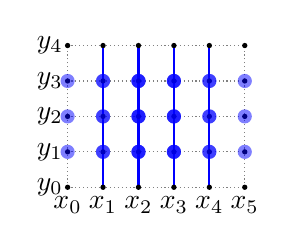
\begin{tikzpicture}[scale=0.45]
                    \foreach \y in {0,...,4} {
                         \draw[gray, densely dotted] (0,\y) -- (5,\y);
                         \node at (-0.5, \y) {$y_{\y}$};
                     } 
                                         
                     \foreach \x in {0,...,5} {
                         \draw[gray, densely dotted] (\x,0) -- (\x,4);
                         \node at (\x, -0.5) {$x_{\x}$};
                         \onslide<2->{
                         \ifnum \x = 1
                            \draw[blue, thick] (1,0) -- (1,4);
                         \fi
                         }
                         \onslide<3->{
                            \ifnum \x = 2
                               \draw[blue, thick] (2,0) -- (2,4);
                            \fi
                         }
                         \onslide<4->{
                            \ifnum \x = 3
                               \draw[blue, thick] (3,0) -- (3,4);
                            \fi
                         }
                            \onslide<5->{
                                \ifnum \x = 4
                                \draw[blue, thick] (4,0) -- (4,4);
                                \fi
                            }
                     }
                     \foreach \x in {0,...,5}
                         \foreach \y in {0,...,4} {
                             \fill (\x,\y) circle (0.0753); 
                             \onslide<2->{
                             \ifnum  \x=0 \ifnum  \y>0 \ifnum  \y<4 
                                 \fill[blue, fill opacity=0.5] (\x,\y) circle (0.2);
                            \fi \fi \fi
                            \ifnum  \x=1 \ifnum  \y>0 \ifnum  \y<4 
                                 \fill[blue, fill opacity=0.5] (\x,\y) circle (0.2);
                            \fi \fi \fi
                            \ifnum  \x=2 \ifnum  \y>0 \ifnum  \y<4 
                                 \fill[blue, fill opacity=0.5] (\x,\y) circle (0.2);
                            \fi \fi \fi
                             } 
                             \onslide<3->{
                                \ifnum  \x=1 \ifnum  \y>0 \ifnum  \y<4
                                    \fill[blue, fill opacity=0.5] (\x,\y) circle (0.2);
                                \fi \fi \fi
                                \ifnum  \x=2 \ifnum  \y>0 \ifnum  \y<4
                                    \fill[blue, fill opacity=0.5] (\x,\y) circle (0.2);
                                \fi \fi \fi
                                \ifnum  \x=3 \ifnum  \y>0 \ifnum  \y<4
                                    \fill[blue, fill opacity=0.5] (\x,\y) circle (0.2);
                                \fi \fi \fi
                                 }
                           \onslide<4->{
                                \ifnum  \x=2 \ifnum  \y>0 \ifnum  \y<4
                                    \fill[blue, fill opacity=0.5] (\x,\y) circle (0.2);
                                \fi \fi \fi
                                \ifnum  \x=3 \ifnum  \y>0 \ifnum  \y<4
                                    \fill[blue, fill opacity=0.5] (\x,\y) circle (0.2);
                                \fi \fi \fi
                                \ifnum  \x=4 \ifnum  \y>0 \ifnum  \y<4
                                    \fill[blue, fill opacity=0.5] (\x,\y) circle (0.2);
                                \fi \fi \fi
                           }
                           \onslide<5->{
                                \ifnum  \x=3 \ifnum  \y>0 \ifnum  \y<4
                                    \fill[blue, fill opacity=0.5] (\x,\y) circle (0.2);
                                \fi \fi \fi
                                \ifnum  \x=4 \ifnum  \y>0 \ifnum  \y<4
                                    \fill[blue, fill opacity=0.5] (\x,\y) circle (0.2);
                                \fi \fi \fi
                                \ifnum  \x=5 \ifnum  \y>0 \ifnum  \y<4
                                    \fill[blue, fill opacity=0.5] (\x,\y) circle (0.2);
                                \fi \fi \fi
                           }
                         }
                         
                 \end{tikzpicture}
                \end{minipage}\\
            \vspace{-0.2cm}
           
            \begin{center}
                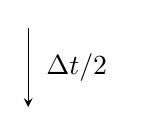
\begin{tikzpicture}[>=stealth]
                    \draw[->] (0,0) -- (0,-1) node[midway, right, xshift=3pt] {$\Delta t/2$};
                \end{tikzpicture}
            \end{center}
            \vspace{-0.2cm}
            \begin{minipage}{0.48\textwidth}
                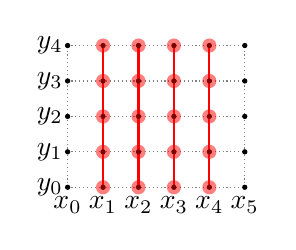
\begin{tikzpicture}[scale=0.45]
                    \foreach \y in {0,...,4} {
                         \draw[gray, densely dotted] (0,\y) -- (5,\y);
                         \node at (-0.5, \y) {$y_{\y}$};
                     }
                                         
                     \foreach \x in {0,...,5} {
                         \draw[gray, densely dotted] (\x,0) -- (\x,4);
                         \node at (\x, -0.5) {$x_{\x}$};
                         \onslide<2->{
                         \ifnum \x = 1
                            \draw[red, thick] (1,0) -- (1,4);
                         \fi}
                        \onslide<3->{
                            \ifnum \x = 2
                               \draw[red, thick] (2,0) -- (2,4);
                            \fi
                        }
                        \onslide<4->{
                            \ifnum \x = 3
                               \draw[red, thick] (3,0) -- (3,4);
                            \fi
                        }
                            \onslide<5->{
                                \ifnum \x = 4
                                \draw[red, thick] (4,0) -- (4,4);
                                \fi
                            }
                     }
                     \foreach \x in {0,...,5}
                         \foreach \y in {0,...,4} {
                             \fill (\x,\y) circle (0.0753); 
                             \onslide<2->{
                             \ifnum \x=1
                            \fill[red, fill opacity=0.5] (\x,\y) circle (0.2);
                            \fi
                            }
                            \onslide<3->{
                                \ifnum \x=2
                                \fill[red, fill opacity=0.5] (\x,\y) circle (0.2);
                                \fi
                            }
                            \onslide<4->{
                                \ifnum \x=3
                                \fill[red, fill opacity=0.5] (\x,\y) circle (0.2);
                                \fi
                            }
                            \onslide<5->{
                                \ifnum \x=4
                                \fill[red, fill opacity=0.5] (\x,\y) circle (0.2);
                                \fi
                            }
                         }
                \end{tikzpicture}
            \end{minipage}
            
        \end{column}
        \hspace{-0.8cm}
       \begin{column}{0.7\textwidth}
            %\footnotesize
            %we need smaller font size. let's try even smaller. Let's try tiny.
            \tiny
          \vspace{-1.5cm}  
          \onslide<2->{
                \begin{align*}
                    \begin{bmatrix}
                        1 + 2\alpha & -\alpha & 0  \\
                         -\alpha & 1 + 2\alpha & -\alpha   \\
                        0 & -\alpha & 1 + 2\alpha   \\
                    \end{bmatrix}
                    \begin{bmatrix}
                        \textcolor{red}{u_{1,1}^{k+1}} \\
                        \textcolor{red}{u_{1,2}^{k+1}} \\
                        \textcolor{red}{u_{1,3}^{k+1}} \\
                    \end{bmatrix}
                    =
                    \begin{bmatrix}
                        \textcolor{blue}{b_{1,1}} \\
                        \textcolor{blue}{b_{1,2}} \\
                        \textcolor{blue}{b_{1,3}} \\
                    \end{bmatrix}
                \end{align*}
          }
                \vspace{-0.5cm}
                \onslide<3->{
                \begin{align*}
                  \begin{bmatrix}
                        1 + 2\alpha & -\alpha & 0  \\
                         -\alpha & 1 + 2\alpha & -\alpha  \\
                        0 & -\alpha & 1 + 2\alpha\\
                    \end{bmatrix}
                    \begin{bmatrix}
                        \textcolor{red}{u_{2,1}^{k+1}} \\
                        \textcolor{red}{u_{2,2}^{k+1}} \\
                        \textcolor{red}{u_{2,3}^{k+1}} \\
                    \end{bmatrix}
                    =
                    \begin{bmatrix}
                        \textcolor{blue}{b_{2,1}} \\
                        \textcolor{blue}{b_{2,2}} \\
                        \textcolor{blue}{b_{2,3}} \\
                    \end{bmatrix}
                \end{align*}
                }
                \vspace{-0.5cm}
                \onslide<4->{
                \begin{align*}
                    \begin{bmatrix}
                        1 + 2\alpha & -\alpha & 0  \\
                         -\alpha & 1 + 2\alpha & -\alpha   \\
                        0 & -\alpha & 1 + 2\alpha\\
                    \end{bmatrix}
                    \begin{bmatrix}
                        \textcolor{red}{u_{3,1}^{k+1}} \\
                        \textcolor{red}{u_{3,2}^{k+1}} \\
                        \textcolor{red}{u_{3,3}^{k+1}} \\
                    \end{bmatrix}
                    =
                    \begin{bmatrix}
                        \textcolor{blue}{b_{3,1}} \\
                        \textcolor{blue}{b_{3,2}} \\
                        \textcolor{blue}{b_{3,3}} \\
                    \end{bmatrix}
                \end{align*}
                } 
                \vspace{-0.5cm}
                \onslide<5->{
                \begin{align*}
                    \begin{bmatrix}
                        1 + 2\alpha & -\alpha & 0  \\
                         -\alpha & 1 + 2\alpha & -\alpha   \\
                        0 & -\alpha & 1 + 2\alpha\\
                    \end{bmatrix}
                    \begin{bmatrix}
                        \textcolor{red}{u_{4,1}^{k+1}} \\
                        \textcolor{red}{u_{4,2}^{k+1}} \\
                        \textcolor{red}{u_{4,3}^{k+1}} \\
                    \end{bmatrix}
                    =
                    \begin{bmatrix}
                        \textcolor{blue}{b_{4,1}} \\
                        \textcolor{blue}{b_{4,2}} \\
                        \textcolor{blue}{b_{4,3}} \\
                    \end{bmatrix}
                \end{align*}
                }
                \vspace{-1.5cm}
        \end{column}
    \end{columns}
   
    \vspace{0.1cm}
    \small
    \onslide<5->{
        Now we can use the Thomas algorithm for solving each individual tridiagonal system.
    }
\end{frame}
\begin{frame}{Adding point-like sinks and sources}
    \vspace{-0.5cm}
    \onslide<1->{
        \begin{align*}
            \frac{\partial u}{\partial t} &= 
            D\Biggl( \frac{\partial^2 u}{\partial x^2} + \frac{\partial^2 u}{\partial y^2} \Biggr) 
            + K_{out} \sum_{p=1}^{N} \delta(r_p - r)
            - K_{in} \sum_{c=1}^{N} \delta(r_c - r)
        \end{align*}
    }
    \onslide<2->{
        We can discretize as follows:
        \vspace{0.5cm}
        {\small % Optionally reduce font size
        \[
        \begin{split}
            \frac{u_{i,j}^{k+\frac{1}{2}} - u_{i,j}^{k}}{\Delta t/2}
            &= D\Biggl(
            \frac{u_{i+1,j}^{k+\frac{1}{2}} - 2u_{i,j}^{k+\frac{1}{2}} + u_{i-1,j}^{k+\frac{1}{2}}}{\Delta x^2} + \frac{u_{i,j+1}^{k} - 2u_{i,j}^{k} + u_{i,j-1}^{k}}{\Delta y^2}
            \Biggr) \\
            \onslide<3->{&\quad + K_{out} \sum_{p=1}^{N} \delta_{\varepsilon}(r_p - r_{i,j})
            - K_{in} \sum_{c=1}^{N} \delta_{\varepsilon}(r_c - r_{i,j}).}
        \end{split}
        \]
        }
        \vspace{0.5cm}
        \onslide<5->{
            We define $\alpha = \frac{D \Delta t}{2\Delta x^2}$ 
            }
            
            \onslide<6->{
            \begin{align*}
                           \resizebox{\textwidth}{!}{%
                $\boxed{\small 
                \colorbox{red!20}{$ -\alpha u_{i-1,j}^{k+\frac{1}{2}} + (1 + 2\alpha)u_{i,j}^{k+\frac{1}{2}} - 
                \alpha u_{i+1,j}^{k+\frac{1}{2}} $}= 
                \colorbox{blue!20}{$\alpha u_{i,j-1}^k + (1 - 2\alpha)u_{i,j}^k + \alpha u_{i,j+1}^k$
                + $K_{out} \sum_{p=1}^{N} \delta_{\varepsilon}(r_p - r_{i,j}) - K_{in} \sum_{c=1}^{N}\delta_{\varepsilon}(r_p - r_{i,j})$}}$}
           \end{align*}
           }
    }
\end{frame}

\begin{frame}
    \begin{align*}
        \resizebox{\textwidth}{!}{%
$\boxed{\small 
\colorbox{red!20}{$ -\alpha u_{i-1,j}^{k+\frac{1}{2}} + (1 + 2\alpha)u_{i,j}^{k+\frac{1}{2}} - 
\alpha u_{i+1,j}^{k+\frac{1}{2}} $}= 
\colorbox{blue!20}{$\alpha u_{i,j-1}^k + (1 - 2\alpha)u_{i,j}^k + \alpha u_{i,j+1}^k$
+ $K_{out} \sum_{p=1}^{N} \delta_{\varepsilon}(r_p - r_{i,j}) - K_{in} \sum_{c=1}^{N}\delta_{\varepsilon}(r_p - r_{i,j})$}}$}
\end{align*}
On the steady state, $\frac{\partial u}{\partial t} = 0$, which means that the difference between the two half-steps is zero:
$\Delta u = u^{k+1/2}_{i,j} - u^{k}_{i,j} = 0$. We can then write the equation as:    
\begin{align*}
    \resizebox{\textwidth}{!}{%
$\boxed{\small 
\colorbox{red!20}{$ -\alpha u_{i-1,j}^{k+\frac{1}{2}}  - 
\alpha u_{i+1,j}^{k+\frac{1}{2}} $}= 
\colorbox{blue!20}{$\alpha u_{i,j-1}^k  - 4\alpha u_{i,j}^k + \alpha u_{i,j+1}^k$
+ $K_{out} \sum_{p=1}^{N} \delta_{\varepsilon}(r_p - r_{i,j}) - K_{in} \sum_{c=1}^{N}\delta_{\varepsilon}(r_p - r_{i,j})$}}$}
\end{align*}
\end{frame}

\end{document}
